% Springer LNCS manuscript. Numbers are injected from generated/macros.tex, which is
% produced by `python -m research_q1.journal.artifacts` from research_q1/outputs/journal-study.json.
\documentclass[runningheads]{llncs}
\usepackage[T1]{fontenc}
\usepackage[utf8]{inputenc}
\usepackage{graphicx}
\usepackage{booktabs}
\usepackage{amsmath,amssymb}
\usepackage{xcolor}
\usepackage[hidelinks]{hyperref}
\usepackage{microtype}
\graphicspath{{generated/figures/}}
% Generated by research_q1.journal.artifacts; do not edit.
\newcommand{\ablDeltaAdsb}{-0.22}
\newcommand{\ablDeltaKin}{-0.19}
\newcommand{\ablDeltaMeta}{+4.86}
\newcommand{\ablDeltaPhys}{+2.58}
\newcommand{\ablDropAdsb}{72.90}
\newcommand{\ablDropKin}{72.93}
\newcommand{\ablDropMeta}{77.98}
\newcommand{\ablDropPhys}{75.70}
\newcommand{\ablFull}{73.12}
\newcommand{\aboveHgbFullMondrianTypeDuration}{0}
\newcommand{\aboveHgbFullSplitConstant}{7}
\newcommand{\aboveHgbFullSplitScaled}{3}
\newcommand{\aboveHgbMetadataAdsbMondrianTypeDuration}{1}
\newcommand{\aboveHgbMetadataAdsbSplitConstant}{8}
\newcommand{\aboveHgbMetadataAdsbSplitScaled}{2}
\newcommand{\aboveHgbResidualPhysicsMondrianTypeDuration}{1}
\newcommand{\aboveHgbResidualPhysicsSplitConstant}{8}
\newcommand{\aboveHgbResidualPhysicsSplitScaled}{1}
\newcommand{\accMaeHgbFullRepresentationFloor}{40.88}
\newcommand{\accMaeHgbFullRiskOnly}{32.42}
\newcommand{\accMaeHgbMetadataAdsbRepresentationFloor}{42.32}
\newcommand{\accMaeHgbMetadataAdsbRiskOnly}{33.23}
\newcommand{\accMaeHgbResidualPhysicsRepresentationFloor}{39.81}
\newcommand{\accMaeHgbResidualPhysicsRiskOnly}{31.98}
\newcommand{\adsbFewHgbFull}{65.31}
\newcommand{\adsbFewHgbMetadataAdsb}{64.80}
\newcommand{\adsbFewHgbResidualPhysics}{61.85}
\newcommand{\adsbManyHgbFull}{55.45}
\newcommand{\adsbManyHgbMetadataAdsb}{57.31}
\newcommand{\adsbManyHgbResidualPhysics}{54.16}
\newcommand{\adsbZeroHgbFull}{123.53}
\newcommand{\adsbZeroHgbMetadataAdsb}{131.71}
\newcommand{\adsbZeroHgbResidualPhysics}{125.85}
\newcommand{\bSevenCovHgbFullRepresentationFloor}{50.0}
\newcommand{\bSevenCovHgbFullRiskOnly}{2.0}
\newcommand{\bSevenCovHgbMetadataAdsbRepresentationFloor}{50.0}
\newcommand{\bSevenCovHgbMetadataAdsbRiskOnly}{0.0}
\newcommand{\bSevenCovHgbResidualPhysicsRepresentationFloor}{50.0}
\newcommand{\bSevenCovHgbResidualPhysicsRiskOnly}{10.2}
\newcommand{\belowHgbFullMondrianTypeDuration}{7}
\newcommand{\belowHgbFullSplitConstant}{15}
\newcommand{\belowHgbFullSplitScaled}{5}
\newcommand{\belowHgbMetadataAdsbMondrianTypeDuration}{6}
\newcommand{\belowHgbMetadataAdsbSplitConstant}{16}
\newcommand{\belowHgbMetadataAdsbSplitScaled}{6}
\newcommand{\belowHgbResidualPhysicsMondrianTypeDuration}{3}
\newcommand{\belowHgbResidualPhysicsSplitConstant}{15}
\newcommand{\belowHgbResidualPhysicsSplitScaled}{4}
\newcommand{\bootReps}{2,000}
\newcommand{\covHgbFullMondrianTypeDuration}{89.6}
\newcommand{\covHgbFullSplitConstant}{90.2}
\newcommand{\covHgbFullSplitScaled}{90.1}
\newcommand{\covHgbMetadataAdsbMondrianTypeDuration}{89.0}
\newcommand{\covHgbMetadataAdsbSplitConstant}{90.6}
\newcommand{\covHgbMetadataAdsbSplitScaled}{89.6}
\newcommand{\covHgbResidualPhysicsMondrianTypeDuration}{89.7}
\newcommand{\covHgbResidualPhysicsSplitConstant}{90.3}
\newcommand{\covHgbResidualPhysicsSplitScaled}{89.6}
\newcommand{\coverageHgbFullRepresentationFloor}{75.0}
\newcommand{\coverageHgbFullRiskOnly}{75.0}
\newcommand{\coverageHgbMetadataAdsbRepresentationFloor}{75.0}
\newcommand{\coverageHgbMetadataAdsbRiskOnly}{75.0}
\newcommand{\coverageHgbResidualPhysicsRepresentationFloor}{75.0}
\newcommand{\coverageHgbResidualPhysicsRiskOnly}{75.0}
\newcommand{\deltaCiHgbFullOct}{[-5.70, -1.03]}
\newcommand{\deltaCiHgbFullSep}{[-9.67, -3.67]}
\newcommand{\deltaCiHgbMetadataOct}{[1.12, 2.78]}
\newcommand{\deltaCiHgbMetadataSep}{[1.40, 3.15]}
\newcommand{\deltaCiHgbResidualPhysicsOct}{[-6.27, -1.35]}
\newcommand{\deltaCiHgbResidualPhysicsSep}{[-11.21, -4.44]}
\newcommand{\deltaCiOpenapCalibratedOct}{[6.06, 12.48]}
\newcommand{\deltaCiOpenapCalibratedSep}{[2.73, 11.30]}
\newcommand{\deltaCiOpenapPhysicsOct}{[48.32, 61.24]}
\newcommand{\deltaCiOpenapPhysicsSep}{[46.39, 61.88]}
\newcommand{\deltaCiTypeMedianRateOct}{[10.59, 14.91]}
\newcommand{\deltaCiTypeMedianRateSep}{[9.85, 15.87]}
\newcommand{\deltaHgbFullOct}{-3.40}
\newcommand{\deltaHgbFullSep}{-6.52}
\newcommand{\deltaHgbMetadataOct}{1.94}
\newcommand{\deltaHgbMetadataSep}{2.23}
\newcommand{\deltaHgbResidualPhysicsOct}{-3.84}
\newcommand{\deltaHgbResidualPhysicsSep}{-7.51}
\newcommand{\deltaOpenapCalibratedOct}{9.08}
\newcommand{\deltaOpenapCalibratedSep}{7.10}
\newcommand{\deltaOpenapPhysicsOct}{54.78}
\newcommand{\deltaOpenapPhysicsSep}{53.95}
\newcommand{\deltaTypeMedianRateOct}{12.78}
\newcommand{\deltaTypeMedianRateSep}{13.06}
\newcommand{\durLongHgbMetadataAdsb}{263.48}
\newcommand{\durLongHgbResidualPhysics}{259.09}
\newcommand{\durMediumHgbMetadataAdsb}{62.88}
\newcommand{\durMediumHgbResidualPhysics}{60.07}
\newcommand{\durShortHgbMetadataAdsb}{46.72}
\newcommand{\durShortHgbResidualPhysics}{42.04}
\newcommand{\eligibleCells}{28}
\newcommand{\flightMapeHgbFull}{26.4}
\newcommand{\flightMapeHgbMetadata}{26.7}
\newcommand{\flightMapeHgbMetadataAdsb}{26.9}
\newcommand{\flightMapeHgbResidualPhysics}{23.1}
\newcommand{\flightMapeOpenapCalibrated}{21.9}
\newcommand{\flightMapeOpenapPhysics}{32.0}
\newcommand{\flightMapeTypeMedianRate}{27.5}
\newcommand{\floorCostHgbFull}{8.46}
\newcommand{\floorCostHgbMetadataAdsb}{9.09}
\newcommand{\floorCostHgbResidualPhysics}{7.83}
\newcommand{\fuelShareHgbFullRepresentationFloor}{42.0}
\newcommand{\fuelShareHgbFullRiskOnly}{26.9}
\newcommand{\fuelShareHgbMetadataAdsbRepresentationFloor}{41.8}
\newcommand{\fuelShareHgbMetadataAdsbRiskOnly}{26.8}
\newcommand{\fuelShareHgbResidualPhysicsRepresentationFloor}{40.6}
\newcommand{\fuelShareHgbResidualPhysicsRiskOnly}{26.3}
\newcommand{\gitCommit}{de6495465c}
\newcommand{\holmHgbFullOct}{0.005}
\newcommand{\holmHgbFullSep}{0.003}
\newcommand{\holmHgbMetadataOct}{0.003}
\newcommand{\holmHgbMetadataSep}{0.003}
\newcommand{\holmHgbResidualPhysicsOct}{0.004}
\newcommand{\holmHgbResidualPhysicsSep}{0.003}
\newcommand{\holmOpenapCalibratedOct}{0.003}
\newcommand{\holmOpenapCalibratedSep}{0.003}
\newcommand{\holmOpenapPhysicsOct}{0.003}
\newcommand{\holmOpenapPhysicsSep}{0.003}
\newcommand{\holmTypeMedianRateOct}{0.003}
\newcommand{\holmTypeMedianRateSep}{0.003}
\newcommand{\invBiasCiHgbFull}{[-2.0, 0.2]}
\newcommand{\invBiasCiHgbMetadata}{[-2.6, 0.1]}
\newcommand{\invBiasCiHgbMetadataAdsb}{[-2.4, 0.2]}
\newcommand{\invBiasCiHgbResidualPhysics}{[-1.9, 0.3]}
\newcommand{\invBiasCiOpenapCalibrated}{[-5.5, -2.8]}
\newcommand{\invBiasCiOpenapPhysics}{[16.0, 19.5]}
\newcommand{\invBiasCiTypeMedianRate}{[-7.4, -4.7]}
\newcommand{\invBiasHgbFull}{-0.8}
\newcommand{\invBiasHgbMetadata}{-1.2}
\newcommand{\invBiasHgbMetadataAdsb}{-1.1}
\newcommand{\invBiasHgbResidualPhysics}{-0.8}
\newcommand{\invBiasOpenapCalibrated}{-4.1}
\newcommand{\invBiasOpenapPhysics}{17.8}
\newcommand{\invBiasTypeMedianRate}{-6.0}
\newcommand{\longCovHgbFullRepresentationFloor}{50.1}
\newcommand{\longCovHgbFullRiskOnly}{1.3}
\newcommand{\longCovHgbMetadataAdsbRepresentationFloor}{50.0}
\newcommand{\longCovHgbMetadataAdsbRiskOnly}{0.7}
\newcommand{\longCovHgbResidualPhysicsRepresentationFloor}{50.0}
\newcommand{\longCovHgbResidualPhysicsRiskOnly}{2.4}
\newcommand{\lotoPooledHgbFull}{111.49}
\newcommand{\lotoPooledHgbMetadata}{181.92}
\newcommand{\lotoPooledHgbMetadataAdsb}{174.68}
\newcommand{\lotoPooledHgbResidualPhysics}{104.40}
\newcommand{\lotoPooledOpenapCalibrated}{98.58}
\newcommand{\lotoPooledOpenapPhysics}{133.07}
\newcommand{\lotoPooledTypeMedianRate}{333.77}
\newcommand{\lotoRelGainHgbFull}{36}
\newcommand{\lotoRelGainHgbMetadata}{-4}
\newcommand{\lotoRelGainHgbMetadataAdsb}{0}
\newcommand{\lotoRelGainHgbResidualPhysics}{40}
\newcommand{\lotoRelGainOpenapCalibrated}{44}
\newcommand{\lotoRelGainOpenapPhysics}{24}
\newcommand{\lotoRelGainTypeMedianRate}{-91}
\newcommand{\lotoTypes}{14}
\newcommand{\lotoWinsHgbFull}{10}
\newcommand{\lotoWinsHgbMetadata}{4}
\newcommand{\lotoWinsHgbMetadataAdsb}{0}
\newcommand{\lotoWinsHgbResidualPhysics}{8}
\newcommand{\lotoWinsOpenapCalibrated}{4}
\newcommand{\lotoWinsOpenapPhysics}{7}
\newcommand{\lotoWinsTypeMedianRate}{1}
\newcommand{\maeCiHgbFullOct}{[68.95, 77.98]}
\newcommand{\maeCiHgbFullSep}{[69.60, 81.31]}
\newcommand{\maeCiHgbMetadataAdsbOct}{[71.66, 82.05]}
\newcommand{\maeCiHgbMetadataAdsbSep}{[74.92, 89.40]}
\newcommand{\maeCiHgbMetadataOct}{[73.56, 84.07]}
\newcommand{\maeCiHgbMetadataSep}{[76.97, 91.92]}
\newcommand{\maeCiHgbResidualPhysicsOct}{[68.53, 77.41]}
\newcommand{\maeCiHgbResidualPhysicsSep}{[68.96, 80.21]}
\newcommand{\maeCiOpenapCalibratedOct}{[80.71, 91.27]}
\newcommand{\maeCiOpenapCalibratedSep}{[82.14, 96.40]}
\newcommand{\maeCiOpenapPhysicsOct}{[124.28, 139.21]}
\newcommand{\maeCiOpenapPhysicsSep}{[125.83, 145.24]}
\newcommand{\maeCiTypeMedianRateOct}{[84.25, 95.05]}
\newcommand{\maeCiTypeMedianRateSep}{[87.83, 102.61]}
\newcommand{\maeHgbFullOct}{73.12}
\newcommand{\maeHgbFullSep}{75.23}
\newcommand{\maeHgbMetadataAdsbOct}{76.52}
\newcommand{\maeHgbMetadataAdsbSep}{81.75}
\newcommand{\maeHgbMetadataOct}{78.47}
\newcommand{\maeHgbMetadataSep}{83.98}
\newcommand{\maeHgbResidualPhysicsOct}{72.68}
\newcommand{\maeHgbResidualPhysicsSep}{74.23}
\newcommand{\maeOpenapCalibratedOct}{85.60}
\newcommand{\maeOpenapCalibratedSep}{88.85}
\newcommand{\maeOpenapPhysicsOct}{131.30}
\newcommand{\maeOpenapPhysicsSep}{135.69}
\newcommand{\maeTypeMedianRateOct}{89.30}
\newcommand{\maeTypeMedianRateSep}{94.81}
\newcommand{\nOct}{37,456}
\newcommand{\nOctFlights}{2,836}
\newcommand{\nSep}{24,289}
\newcommand{\nSepFlights}{1,888}
\newcommand{\nTrain}{131,530}
\newcommand{\nTrainFlights}{11,037}
\newcommand{\nTypes}{26}
\newcommand{\relGainHgbFullOct}{4.4}
\newcommand{\relGainHgbMetadataAdsbOct}{0.0}
\newcommand{\relGainHgbMetadataOct}{-2.5}
\newcommand{\relGainHgbResidualPhysicsOct}{5.0}
\newcommand{\relGainOpenapCalibratedOct}{-11.9}
\newcommand{\relGainOpenapPhysicsOct}{-71.6}
\newcommand{\relGainTypeMedianRateOct}{-16.7}
\newcommand{\rmseHgbFullOct}{217.52}
\newcommand{\rmseHgbFullSep}{233.49}
\newcommand{\rmseHgbMetadataAdsbOct}{226.12}
\newcommand{\rmseHgbMetadataAdsbSep}{254.33}
\newcommand{\rmseHgbMetadataOct}{233.14}
\newcommand{\rmseHgbMetadataSep}{263.07}
\newcommand{\rmseHgbResidualPhysicsOct}{211.99}
\newcommand{\rmseHgbResidualPhysicsSep}{220.19}
\newcommand{\rmseOpenapCalibratedOct}{250.04}
\newcommand{\rmseOpenapCalibratedSep}{266.87}
\newcommand{\rmseOpenapPhysicsOct}{338.00}
\newcommand{\rmseOpenapPhysicsSep}{368.22}
\newcommand{\rmseTypeMedianRateOct}{249.36}
\newcommand{\rmseTypeMedianRateSep}{266.59}
\newcommand{\rsqHgbFullOct}{0.920}
\newcommand{\rsqHgbFullSep}{0.909}
\newcommand{\rsqHgbMetadataAdsbOct}{0.914}
\newcommand{\rsqHgbMetadataAdsbSep}{0.892}
\newcommand{\rsqHgbMetadataOct}{0.909}
\newcommand{\rsqHgbMetadataSep}{0.885}
\newcommand{\rsqHgbResidualPhysicsOct}{0.924}
\newcommand{\rsqHgbResidualPhysicsSep}{0.919}
\newcommand{\rsqOpenapCalibratedOct}{0.895}
\newcommand{\rsqOpenapCalibratedSep}{0.881}
\newcommand{\rsqOpenapPhysicsOct}{0.808}
\newcommand{\rsqOpenapPhysicsSep}{0.774}
\newcommand{\rsqTypeMedianRateOct}{0.895}
\newcommand{\rsqTypeMedianRateSep}{0.881}
\newcommand{\runtimeMin}{3.3}
\newcommand{\seenRouteHgbFull}{67.84}
\newcommand{\seenRouteHgbMetadata}{72.55}
\newcommand{\seenRouteHgbMetadataAdsb}{70.75}
\newcommand{\seenRouteHgbResidualPhysics}{67.65}
\newcommand{\seenRouteN}{35,422}
\newcommand{\seenRouteOpenapCalibrated}{80.58}
\newcommand{\seenRouteOpenapPhysics}{122.56}
\newcommand{\seenRouteTypeMedianRate}{84.09}
\newcommand{\shortOct}{46.2}
\newcommand{\spearmanHgbFull}{0.603}
\newcommand{\spearmanHgbMetadataAdsb}{0.604}
\newcommand{\spearmanHgbResidualPhysics}{0.613}
\newcommand{\unitAlt}{37,000}
\newcommand{\unitGs}{449}
\newcommand{\unseenRouteHgbFull}{165.01}
\newcommand{\unseenRouteHgbMetadata}{181.52}
\newcommand{\unseenRouteHgbMetadataAdsb}{177.12}
\newcommand{\unseenRouteHgbResidualPhysics}{160.24}
\newcommand{\unseenRouteN}{2,034}
\newcommand{\unseenRouteOpenapCalibrated}{173.00}
\newcommand{\unseenRouteOpenapPhysics}{283.52}
\newcommand{\unseenRouteTypeMedianRate}{180.07}
\newcommand{\widthHgbFullMondrianTypeDuration}{321}
\newcommand{\widthHgbFullSplitConstant}{273}
\newcommand{\widthHgbFullSplitScaled}{350}
\newcommand{\widthHgbMetadataAdsbMondrianTypeDuration}{329}
\newcommand{\widthHgbMetadataAdsbSplitConstant}{289}
\newcommand{\widthHgbMetadataAdsbSplitScaled}{343}
\newcommand{\widthHgbResidualPhysicsMondrianTypeDuration}{320}
\newcommand{\widthHgbResidualPhysicsSplitConstant}{274}
\newcommand{\widthHgbResidualPhysicsSplitScaled}{332}
\newcommand{\winklerHgbFullMondrianTypeDuration}{518}
\newcommand{\winklerHgbFullSplitConstant}{776}
\newcommand{\winklerHgbFullSplitScaled}{541}
\newcommand{\winklerHgbMetadataAdsbMondrianTypeDuration}{569}
\newcommand{\winklerHgbMetadataAdsbSplitConstant}{824}
\newcommand{\winklerHgbMetadataAdsbSplitScaled}{577}
\newcommand{\winklerHgbResidualPhysicsMondrianTypeDuration}{510}
\newcommand{\winklerHgbResidualPhysicsSplitConstant}{775}
\newcommand{\winklerHgbResidualPhysicsSplitScaled}{528}
\newcommand{\worstHgbFullMondrianTypeDuration}{69.4}
\newcommand{\worstHgbFullSplitConstant}{25.6}
\newcommand{\worstHgbFullSplitScaled}{72.8}
\newcommand{\worstHgbMetadataAdsbMondrianTypeDuration}{68.8}
\newcommand{\worstHgbMetadataAdsbSplitConstant}{29.4}
\newcommand{\worstHgbMetadataAdsbSplitScaled}{63.8}
\newcommand{\worstHgbResidualPhysicsMondrianTypeDuration}{67.6}
\newcommand{\worstHgbResidualPhysicsSplitConstant}{23.3}
\newcommand{\worstHgbResidualPhysicsSplitScaled}{78.9}
\newcommand{\zeroAdsbOct}{25.5}

\renewcommand\UrlFont{\color{blue}\rmfamily}
\setlength{\emergencystretch}{1.5em}

\begin{document}

\title{Physics-Informed Fuel Estimation from Open ADS-B Data with Group-Conditional Uncertainty and Representation-Aware Release}
\titlerunning{Physics-Informed Fuel Estimation with Representation-Aware Release}

\author{Anonymous Author(s)\inst{1}\orcidID{0000-0000-0000-0000}}
\authorrunning{Anonymous et al.}
\institute{Institution withheld for review\\
\email{withheld@example.org}}

\maketitle

\begin{abstract}
Open ADS-B surveillance enables large-scale aircraft fuel estimation, but aggregate accuracy hides three questions that matter for research use: whether a physics prior improves transfer to under-represented aircraft, whether uncertainty statements hold inside aircraft-type and duration cells, and how many hard cases are silently dropped when only ``reliable'' estimates are released.
We study these questions on the EUROCONTROL PRC~2025 benchmark (\nTrain{} training, \nSep{} calibration and \nOct{} forward-test intervals from \nTypes{} aircraft types) under a strictly chronological, flight-disjoint protocol.
We derive SI kinematic and OpenAP physics features from raw trajectories after correcting a unit discrepancy in the published documentation, and compare seven estimators from a type-median rate to a physics-residual gradient-boosting model.
On October~2025 the physics-residual model reaches \maeHgbResidualPhysicsOct{}\,kg MAE versus \maeHgbMetadataAdsbOct{}\,kg for the inherited metadata+ADS-B model (paired flight-cluster bootstrap difference \deltaHgbResidualPhysicsOct{}\,kg, 95\% CI \deltaCiHgbResidualPhysicsOct{}); refit ablation attributes the gain to the OpenAP physics features rather than to additional kinematic summaries.
In leave-one-aircraft-type-out refits over \lotoTypes{} types, the physics-informed learners beat the reference on \lotoWinsHgbFull{} (HGB full) and \lotoWinsHgbResidualPhysics{} (physics-residual) types and cut pooled held-out MAE from \lotoPooledHgbMetadataAdsb{} to \lotoPooledHgbResidualPhysics{}\,kg.
Nominal 90\% split-conformal intervals with constant width keep \covHgbFullSplitConstant{}\% marginal coverage but under-cover \belowHgbFullSplitConstant{} of \eligibleCells{} aircraft-type$\times$duration cells (worst \worstHgbFullSplitConstant{}\%); error-scaled and hierarchical Mondrian intervals reduce this to \belowHgbFullSplitScaled{} and \belowHgbFullMondrianTypeDuration{} cells, but no method reaches 85\% in every cell under the September-to-October shift.
At a fixed 75\% release rate, guaranteeing 50\% release in every duration bin and frequent aircraft type raises the share of labelled fuel represented from \fuelShareHgbResidualPhysicsRiskOnly{}\% to \fuelShareHgbResidualPhysicsRepresentationFloor{}\% at a cost of \floorCostHgbResidualPhysics{}\,kg accepted MAE.
All code, configuration hashes and result files are released; the study is a forward temporal evaluation on development-era data and not an external validation.
\keywords{Aircraft fuel burn \and ADS-B \and Physics-informed machine learning \and Conformal prediction \and Selective regression \and Open aviation data.}
\end{abstract}

\section{Introduction}
Fuel burn is the dominant driver of aviation operating cost and CO$_2$ emissions, yet measured fuel data remain proprietary. Open surveillance data from the OpenSky Network~\cite{schafer2014opensky} make scalable estimation possible, and the EUROCONTROL PRC~2025 Data Challenge~\cite{sun2026prc,zenodo_prc2025} released the first large public benchmark that pairs ACARS fuel-on-board differences with ADS-B trajectories for 15,761 flights.
Challenge entries showed that physics-guided gradient boosting with OpenAP~\cite{sun2020openap} features and meteorology is highly competitive~\cite{grigoriou2026physics,kacar2026weather}.

Accuracy on a random or pooled test set, however, does not answer the questions that arise when such estimates are consumed downstream. A curator building an emissions inventory needs to know whether the estimator transfers to aircraft types rarely seen in training; a researcher reporting uncertainty needs intervals that are valid \emph{within} aircraft and duration groups, not only on average~\cite{vovk2012mondrian,gibbs2023conditional}; and anyone who filters estimates by predicted reliability needs to know which flights disappear, because selective regression is known to magnify subgroup disparities~\cite{shah2022selective}.
Our earlier audit of this benchmark (released in the same repository) had already shown, with a metadata-and-ADS-B model, that risk-only release of 75\% of late-September intervals retained fewer than 1\% of 15--60-minute intervals and one of 66 Boeing 747-400 intervals.

This paper makes the following contributions.
\begin{enumerate}
  \item We document and correct a unit discrepancy in the PRC~2025 trajectory release (feet, knots and ft/min rather than the documented metres and m/s) and derive SI kinematic, energy-rate and OpenAP fuel-flow features from the raw ADS-B rows only (Sect.~\ref{sec:data}).
  \item We compare seven estimators under one pre-registered configuration (Sect.~\ref{sec:methods}), including a physics-residual model that learns corrections to a type-scaled OpenAP prior, and test them with paired flight-cluster bootstrap inference and Holm correction~\cite{holm1979} on a forward October test (Sect.~\ref{sec:results}).
  \item We quantify transfer to withheld aircraft types with leave-one-type-out refits and to unseen routes.
  \item We evaluate constant, $\hat\sigma$-scaled and hierarchical Mondrian conformal intervals cell-by-cell, and
  \item we measure the accuracy cost of a representation floor across a release frontier for each estimator, so that the access--accuracy trade-off can be read together with the point and interval results.
\end{enumerate}
We do not claim a new learning algorithm or a conformal theorem. The contribution is an auditable, jointly evaluated estimation--uncertainty--release pipeline on open data, with every number in this paper generated from a committed result file.

\section{Data and Leakage Controls}\label{sec:data}
\paragraph{Benchmark.}
The PRC~2025 dataset~\cite{zenodo_prc2025} provides, for each flight, metadata (aircraft type, take-off and landing times, origin and destination), a trajectory file fusing ADS-B positions with sparse ACARS reports, and labelled intervals whose target \texttt{fuel\_kg} is the difference between consecutive ACARS fuel-on-board reports. Splits are chronological by construction: April--August (training), September (``rank'') and October~2025 (``final''). All downloads were verified against the publisher's MD5 checksums.

\paragraph{Unit correction.}
The published README states that altitude, ground speed and vertical rate are in metres, m/s and m/s. Across all flights, the median per-flight 90th-percentile altitude when ground speed exceeds 300 is \unitAlt{} and the median ground speed is \unitGs{}; these are only plausible as feet and knots. We therefore convert to SI before any physics computation and report this as a correction to the dataset documentation. Out-of-range raw values are set to missing, and position spikes implying ground speeds above $\sim$680\,kt are excluded from along-track distance (Sect.~\ref{sec:features}).

\paragraph{Leakage controls.}
Only rows with \texttt{source = adsb} enter any feature; ACARS rows, which carry the labels, are discarded before aggregation. All models and the per-type physics scale factors are fit on April--August only. September is split by a stable hash of the flight identifier into two flight-disjoint halves: half~A fits the error model $\hat\sigma$, half~B provides conformal calibration. October is used once, for evaluation. Train, calibration and test flight identifiers are checked to be disjoint. October aggregates had been inspected during development of the inherited metadata+ADS-B model, so we describe October as a forward temporal test on development-era data, not a sealed confirmatory set.

\section{Methods}\label{sec:methods}
\subsection{Features}\label{sec:features}
Four feature groups are used. \emph{Metadata} (7): interval duration, whole-flight duration, elapsed time from take-off, remaining time to landing, hour-of-day encoding and great-circle route distance from the airport table. \emph{ADS-B summaries} (14): the inherited position/speed counts, raw altitude/speed/vertical-rate quantiles and gap statistics. \emph{SI kinematics} (14): mean and change in altitude and ground speed, mean vertical rate, climb/descent/ground fractions, spike-filtered along-track distance, observed-span fraction, the specific-energy rate $\big(g\,\Delta h + \tfrac12\Delta v^2\big)/\Delta t$, and interpolated altitude and speed at the interval boundaries. \emph{Physics} (3): the OpenAP fuel-flow model~\cite{sun2020openap} integrated at 30-second steps over the interval using a nominal mass $m_{\mathrm{OEW}} + 0.5\,(m_{\mathrm{MTOW}}-m_{\mathrm{OEW}})$, ground speed as a proxy for true airspeed (winds are unavailable), a 7\%-of-static-thrust ground fuel flow when ground speed is below 40\,m/s, the fraction of ground samples and the largest interpolation gap. Types absent from OpenAP use the library's documented synonyms. The nominal mass and wind-free airspeed are deliberate, documented approximations; the learned models are expected to absorb their bias.

\subsection{Estimators}
Let $y_i$ be the labelled fuel of interval $i$ and $x_i$ its features. We compare
(i) \emph{type median rate}: duration $\times$ training median kg/min per aircraft type;
(ii) \emph{OpenAP physics}: the integrated fuel flow $\phi_i$ without calibration;
(iii) \emph{OpenAP type-scaled}: $s_{t(i)}\,\phi_i$ with $s_t=\sum_i y_i\phi_i/\sum_i\phi_i^2$ over training intervals of type $t$;
(iv--vi) histogram gradient boosting (HGB) on metadata, metadata+ADS-B (the inherited reference), and all four groups (\emph{HGB full}); and
(vii) \emph{physics-residual HGB}: $\hat y_i = s_{t(i)}\phi_i + g(x_i)$ where $g$ is an HGB model fit to $y_i - s_{t(i)}\phi_i$ on all feature groups.
Physics features are computed by interpolating the flight's ADS-B states at the sample times, so an interval without positions of its own still receives a prior from neighbouring observations; the largest interpolation gap is kept as a feature so that the learners can discount such cases. The type median rate is used only if a flight has fewer than two valid ADS-B positions. Hyperparameters (400 trees, learning rate 0.05, 31 leaves, $\ell_2=10$) were copied from the inherited configuration and not tuned on any evaluation period; all predictions are clipped at zero.

\subsection{Error model, intervals and release}
For each point model an HGB error model $\hat\sigma(x)$ is fit on September half~A to the absolute residuals using the full feature set plus the log prediction. On half~B we compute conformity scores $r_i=|y_i-\hat y_i|/\hat\sigma(x_i)$ and compare three nominal 90\% procedures: constant-width split conformal (quantile of $|y_i-\hat y_i|$), $\hat\sigma$-scaled split conformal (quantile of $r_i$), and a hierarchical Mondrian procedure~\cite{vovk2012mondrian} that takes the finite-sample quantile of $r_i$ within aircraft-type$\times$duration-bin cells with at least 50 calibration rows, falling back to the aircraft type, then the duration bin, then the global quantile. Coverage is evaluated on October in every cell with at least 100 test intervals, with flight-cluster bootstrap intervals.

Release follows the inherited deterministic rule: intervals are ranked by $\hat\sigma$; a floor $f$ forces at least $\lceil f\,n_g\rceil$ releases in each duration bin $g$ and each aircraft type with at least 50 intervals in the batch, and the remaining budget up to the overall target is filled by lowest $\hat\sigma$. We compare $f=0$ (risk ranking only) with $f=0.5$ at targets from 50\% to 100\%, reporting accepted and rejected MAE, the share of labelled fuel represented and group release rates. Labels are used only after selection.

\subsection{Statistics}
MAE differences against the reference are tested with a paired bootstrap that resamples whole flights (\bootReps{} repetitions), reporting percentile 95\% CIs and two-sided bootstrap $p$-values, Holm-adjusted across the six comparisons per period~\cite{holm1979}. Leave-one-type-out (LOTO) refits all estimators and scale factors without one aircraft type and evaluates on that type's September and October intervals, for every type with at least 200 evaluation intervals. Flight-level totals and inventory bias use flight-cluster bootstraps. Configuration, code and source-file SHA-256 hashes, package versions and the git commit are recorded in the result file (commit \texttt{\gitCommit}, runtime \runtimeMin{}\,min).

\section{Results}\label{sec:results}
\subsection{Point prediction}
Table~\ref{tab:models} and Fig.~\ref{fig:models} compare the seven estimators. The uncalibrated OpenAP prior alone reaches \maeOpenapPhysicsOct{}\,kg on October and overestimates labelled inventory by \invBiasOpenapPhysics{}\%, consistent with a nominal mass and wind-free airspeed; per-type scaling reduces its MAE to \maeOpenapCalibratedOct{}\,kg, \deltaOpenapCalibratedOct{}\,kg from the learned reference (\maeHgbMetadataAdsbOct{}\,kg). Adding SI kinematics and physics to the reference (HGB full) changes October MAE by \deltaHgbFullOct{}\,kg (95\% CI \deltaCiHgbFullOct{}, Holm $p$ = \holmHgbFullOct). The physics-residual model gives the largest improvement, \deltaHgbResidualPhysicsOct{}\,kg (95\% CI \deltaCiHgbResidualPhysicsOct{}, Holm $p$ = \holmHgbResidualPhysicsOct), with October RMSE \rmseHgbResidualPhysicsOct{}\,kg and $R^2$ = \rsqHgbResidualPhysicsOct. September shows the same ordering with larger gains (\deltaHgbResidualPhysicsSep{}\,kg, 95\% CI \deltaCiHgbResidualPhysicsSep{}). The improvements are a few percent of MAE: statistically clear, but modest relative to the remaining error.

\begin{table}[t]
\centering
\caption{Point-prediction results. MAE confidence intervals resample whole flights; $\Delta$MAE is the paired difference against the metadata+ADS-B reference (negative favours the row model).}
\label{tab:models}
\scriptsize
\setlength{\tabcolsep}{3pt}
\resizebox{\linewidth}{!}{\begin{tabular}{lrrlrrl}
\toprule
Model & Sep.\ MAE & Oct.\ MAE & Oct.\ MAE 95\% CI & Oct.\ RMSE & Oct.\ $R^2$ & $\Delta$MAE vs.\ ref.\ [95\% CI] \\
 & (kg) & (kg) & (kg) & (kg) & & (kg) \\
\midrule
Type median rate & 94.81 & 89.30 & [84.25, 95.05] & 249.36 & 0.895 & +12.78 [10.59, 14.91] \\
OpenAP physics (uncalibrated) & 135.69 & 131.30 & [124.28, 139.21] & 338.00 & 0.808 & +54.78 [48.32, 61.24] \\
OpenAP physics (type-scaled) & 88.85 & 85.60 & [80.71, 91.27] & 250.04 & 0.895 & +9.08 [6.06, 12.48] \\
HGB metadata & 83.98 & 78.47 & [73.56, 84.07] & 233.14 & 0.909 & +1.94 [1.12, 2.78] \\
HGB metadata + ADS-B summaries & 81.75 & 76.52 & [71.66, 82.05] & 226.12 & 0.914 & reference \\
HGB full (+ kinematics + physics) & 75.23 & 73.12 & [68.95, 77.98] & 217.52 & 0.920 & -3.40 [-5.70, -1.03] \\
Physics-residual HGB & 74.23 & 72.68 & [68.53, 77.41] & 211.99 & 0.924 & -3.84 [-6.27, -1.35] \\
\bottomrule
\end{tabular}
}
\end{table}

\begin{figure}[t]
\centering
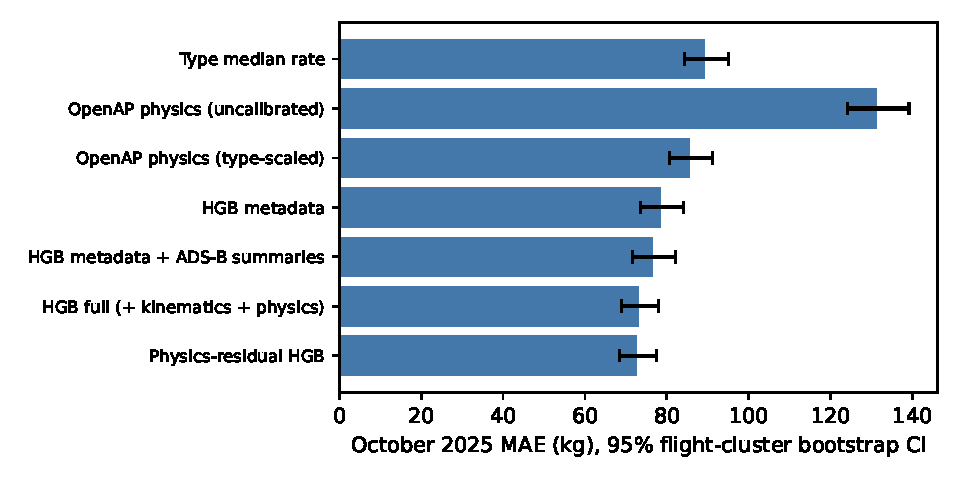
\includegraphics[width=\linewidth]{model_comparison.pdf}
\caption{October 2025 MAE by estimator with 95\% flight-cluster bootstrap intervals.}
\label{fig:models}
\end{figure}

\paragraph{Ablation.}
Removing feature groups from HGB full (Table~\ref{tab:ablation}) shows where the gain comes from: dropping the three physics features raises October MAE by \ablDeltaPhys{}\,kg and dropping flight metadata by \ablDeltaMeta{}\,kg, whereas dropping the 14 SI kinematic features (\ablDeltaKin{}\,kg) or the 14 original ADS-B summaries (\ablDeltaAdsb{}\,kg) changes it by less than half a kilogram. Given the physics prior, raw kinematic summaries are therefore largely redundant. These are refit ablations on one configuration; they describe predictive contribution, not causal effect.

\begin{table}[t]
\centering
\caption{Refit feature-group ablation of HGB full on October 2025.}
\label{tab:ablation}
\scriptsize
\begin{tabular}{lrr}
\toprule
Removed feature group & Oct.\ MAE (kg) & $\Delta$ vs.\ full (kg) \\
\midrule
None (full model) & 73.12 & 0.00 \\
Original ADS-B summaries (14) & 72.90 & -0.22 \\
SI kinematics and energy (14) & 72.93 & -0.19 \\
Flight metadata (duration, timing, route distance) & 77.98 & +4.86 \\
OpenAP physics (3) & 75.70 & +2.58 \\
\bottomrule
\end{tabular}

\end{table}

\paragraph{Subgroups and data availability.}
Table~\ref{tab:subgroups} reports October MAE by duration bin, ADS-B availability and the most frequent aircraft types. \zeroAdsbOct{}\% of October intervals have no ADS-B position inside the interval. For these, the in-interval summaries are missing and the physics prior relies on interpolation across the gap; their MAE is \adsbZeroHgbResidualPhysics{}\,kg for the physics-residual model and \adsbZeroHgbMetadataAdsb{}\,kg for the reference, against \adsbManyHgbResidualPhysics{} and \adsbManyHgbMetadataAdsb{}\,kg for intervals with more than 50 positions. Error rises steeply with duration (15--60\,min: \durLongHgbResidualPhysics{}\,kg versus \durShortHgbResidualPhysics{}\,kg below five minutes), so pooled MAE is dominated by long intervals.

\begin{table}[t]
\centering
\caption{October 2025 MAE (kg) by subgroup. ADS-B availability counts positions inside the interval.}
\label{tab:subgroups}
\scriptsize
\setlength{\tabcolsep}{3pt}
\resizebox{\linewidth}{!}{\begin{tabular}{lrrrrrr}
\toprule
Group & $n$ & Type median rate & OpenAP scaled & HGB meta+ADS-B & HGB full & Physics-residual HGB \\
\midrule
\multicolumn{7}{l}{\emph{Duration}} \\
\quad $<$5 min & 17,318 & 51.15 & 47.04 & 46.72 & 43.10 & 42.04 \\
\quad 5--15 min & 16,195 & 76.26 & 69.98 & 62.88 & 60.58 & 60.07 \\
\quad 15--60 min & 3,943 & 310.45 & 319.17 & 263.48 & 256.49 & 259.09 \\
\multicolumn{7}{l}{\emph{ADS-B positions}} \\
\quad zero & 9,557 & 134.99 & 157.14 & 131.71 & 123.53 & 125.85 \\
\quad 1-50 & 1,136 & 53.87 & 74.21 & 64.80 & 65.31 & 61.85 \\
\quad 51+ & 26,763 & 74.49 & 60.54 & 57.31 & 55.45 & 54.16 \\
\multicolumn{7}{l}{\emph{Aircraft type (October $n \geq 200$)}} \\
\quad A20N & 17,095 & 42.92 & 43.08 & 39.27 & 38.21 & 38.20 \\
\quad A320 & 8,042 & 65.79 & 48.31 & 42.93 & 41.27 & 40.41 \\
\quad A359 & 5,592 & 171.29 & 177.36 & 136.35 & 134.20 & 136.21 \\
\quad A332 & 1,396 & 158.05 & 142.16 & 145.83 & 129.84 & 129.03 \\
\quad B738 & 1,319 & 92.33 & 65.72 & 58.48 & 56.29 & 54.29 \\
\quad B789 & 807 & 144.13 & 169.65 & 140.91 & 122.06 & 130.64 \\
\quad A21N & 805 & 48.38 & 59.71 & 40.27 & 50.20 & 43.63 \\
\quad B77W & 713 & 409.30 & 420.55 & 474.41 & 450.05 & 452.23 \\
\quad B788 & 350 & 145.33 & 117.21 & 183.43 & 109.24 & 109.66 \\
\quad B744 & 342 & 393.35 & 467.09 & 383.05 & 418.79 & 373.44 \\
\quad A333 & 336 & 158.66 & 144.81 & 176.87 & 142.35 & 138.22 \\
\quad A319 & 221 & 56.83 & 30.75 & 44.07 & 38.88 & 31.72 \\
\bottomrule
\end{tabular}
}
\end{table}

\subsection{Transfer to withheld aircraft types and unseen routes}
Table~\ref{tab:loto} gives LOTO results for the \lotoTypes{} aircraft types with at least 200 evaluation intervals. HGB full beats the reference on \lotoWinsHgbFull{} types and the physics-residual model on \lotoWinsHgbResidualPhysics{}; pooled held-out MAE falls from \lotoPooledHgbMetadataAdsb{}\,kg (reference) to \lotoPooledHgbFull{} and \lotoPooledHgbResidualPhysics{}\,kg, and the simple type-scaled OpenAP prior, which wins only \lotoWinsOpenapCalibrated{} individual types, has the lowest pooled value (\lotoPooledOpenapCalibrated{}\,kg) because it avoids the largest failures on the most frequent types. Even the uncalibrated prior beats the reference on \lotoWinsOpenapPhysics{} held-out types, mostly narrow-bodies. The gains are largest for types whose closest training relatives differ in size or engines (e.g.\ A20N, B744, B788); for types with a close sibling in training (A21N, B738, A359) the reference remains competitive or better. When a type is unseen, its one-hot indicator is all zeros and the reference can only borrow from superficially similar types, whereas the physics prior carries type-specific engine and drag information from OpenAP. For an unseen type the scale factor $s_t$ falls back to the global scale, so the physics models' calibration is type-agnostic in these tests.

\begin{table}[t]
\centering
\caption{Leave-one-aircraft-type-out MAE (kg) on the held-out type's September and October intervals. Bold marks the best model per row. The reference is HGB metadata+ADS-B.}
\label{tab:loto}
\scriptsize
\setlength{\tabcolsep}{3pt}
\resizebox{\linewidth}{!}{\begin{tabular}{lrrrrrrr}
\toprule
Held-out type & $n$ & Type rate & OpenAP & OpenAP scaled & HGB meta+ADS-B & HGB full & Physics-residual \\
\midrule
A20N & 29,084 & 284.82 & 52.77 & \textbf{40.50} & 197.36 & 76.43 & 56.20 \\
A21N & 954 & \textbf{48.46} & 61.63 & 81.72 & 60.19 & 62.07 & 67.88 \\
A319 & 345 & 56.24 & \textbf{33.04} & 63.53 & 45.86 & 37.76 & 49.62 \\
A320 & 13,035 & 70.87 & \textbf{46.80} & 70.43 & 66.45 & 50.48 & 63.37 \\
A321 & 307 & 134.59 & 125.37 & 132.17 & \textbf{78.32} & 79.84 & 80.05 \\
A332 & 2,201 & 362.32 & \textbf{169.68} & 218.51 & 217.49 & 173.06 & 200.19 \\
A333 & 527 & 369.40 & \textbf{140.41} & 200.74 & 188.61 & 140.84 & 182.35 \\
A359 & 9,170 & 731.44 & 371.24 & 193.27 & \textbf{182.59} & 240.48 & 219.07 \\
B738 & 1,904 & 88.01 & \textbf{58.55} & 91.75 & 59.99 & 63.38 & 81.43 \\
B744 & 582 & 1,367.38 & 966.02 & 547.04 & 879.87 & 551.37 & \textbf{464.60} \\
B772 & 220 & 1,137.08 & 1,221.94 & 597.11 & 349.72 & \textbf{333.35} & 518.54 \\
B77W & 1,031 & 1,117.30 & 673.14 & 422.70 & 599.48 & \textbf{382.51} & 408.41 \\
B788 & 737 & 401.28 & \textbf{136.20} & 222.05 & 354.73 & 144.78 & 204.14 \\
B789 & 1,437 & 600.83 & 240.77 & 171.97 & 146.27 & 143.82 & \textbf{139.73} \\
\midrule
Pooled & 61,534 & 333.77 & 133.07 & 98.58 & 174.68 & 111.49 & 104.40 \\
Types beating reference & & 1 & 7 & 4 & -- & 10 & 8 \\
\bottomrule
\end{tabular}
}
\end{table}

On October intervals from routes present in training (\seenRouteN{} intervals) versus unseen routes (\unseenRouteN{}), the reference has \seenRouteHgbMetadataAdsb{} vs.\ \unseenRouteHgbMetadataAdsb{}\,kg MAE and the physics-residual model \seenRouteHgbResidualPhysics{} vs.\ \unseenRouteHgbResidualPhysics{}\,kg. The seen/unseen comparison is confounded by aircraft and duration mix and is reported descriptively.

\subsection{Group-conditional uncertainty}
Table~\ref{tab:intervals} and Fig.~\ref{fig:cells} evaluate nominal 90\% intervals on October. For HGB full, all three methods are close to nominal marginally (\covHgbFullSplitConstant{}, \covHgbFullSplitScaled{} and \covHgbFullMondrianTypeDuration{}\%), which is precisely why marginal coverage is uninformative here. Constant-width split conformal under-covers \belowHgbFullSplitConstant{} of \eligibleCells{} cells (worst \worstHgbFullSplitConstant{}\%, long B77W intervals) and over-covers \aboveHgbFullSplitConstant{} narrow-body cells above 97\%. Scaling by the learned error model (Spearman correlation with realised error \spearmanHgbFull{}; Fig.~\ref{fig:deciles}) does most of the repair: \belowHgbFullSplitScaled{} cells below 85\%, worst \worstHgbFullSplitScaled{}\%, mean width \widthHgbFullSplitScaled{}\,kg. Hierarchical Mondrian calibration leaves \belowHgbFullMondrianTypeDuration{} cells below 85\% and \aboveHgbFullMondrianTypeDuration{} above 97\% at a narrower mean width of \widthHgbFullMondrianTypeDuration{}\,kg, but its worst cell (\worstHgbFullMondrianTypeDuration{}\%) is not better than the scaled method's. The remaining failures concentrate in A21N, A333, B788 and B77W cells, where the September calibration cells are small and the October error distribution has shifted. Because September and October are not exchangeable, these are empirical coverages, not guarantees; our pre-registered expectation that Mondrian calibration would reach 85\% in every cell (H3) is not supported.

\begin{table}[t]
\centering
\caption{Nominal 90\% interval results on October 2025. Cells are aircraft type $\times$ duration bin with $\geq 100$ test intervals.}
\label{tab:intervals}
\scriptsize
\setlength{\tabcolsep}{3pt}
\resizebox{\linewidth}{!}{\begin{tabular}{llrrrrr}
\toprule
Point model & Interval method & Coverage & Width & Winkler & Worst cell & Cells \\
 & & (\%) & (kg) & (kg) & cov.\ (\%) & $<85\%$ \\
\midrule
HGB full (+ kinematics + physics) & Hierarchical Mondrian (type $\times$ duration) & 89.6 & 321 & 518 & 69.4 & 7 \\
HGB full (+ kinematics + physics) & Split conformal (constant width) & 90.2 & 273 & 776 & 25.6 & 15 \\
HGB full (+ kinematics + physics) & Split conformal ($\hat\sigma$-scaled) & 90.1 & 350 & 541 & 72.8 & 5 \\
HGB metadata + ADS-B summaries & Hierarchical Mondrian (type $\times$ duration) & 89.0 & 329 & 569 & 68.8 & 6 \\
HGB metadata + ADS-B summaries & Split conformal (constant width) & 90.6 & 289 & 824 & 29.4 & 16 \\
HGB metadata + ADS-B summaries & Split conformal ($\hat\sigma$-scaled) & 89.6 & 343 & 577 & 63.8 & 6 \\
Physics-residual HGB & Hierarchical Mondrian (type $\times$ duration) & 89.7 & 320 & 510 & 67.6 & 3 \\
Physics-residual HGB & Split conformal (constant width) & 90.3 & 274 & 775 & 23.3 & 15 \\
Physics-residual HGB & Split conformal ($\hat\sigma$-scaled) & 89.6 & 332 & 528 & 78.9 & 4 \\
\bottomrule
\end{tabular}
}
\end{table}

\begin{figure}[t]
\centering
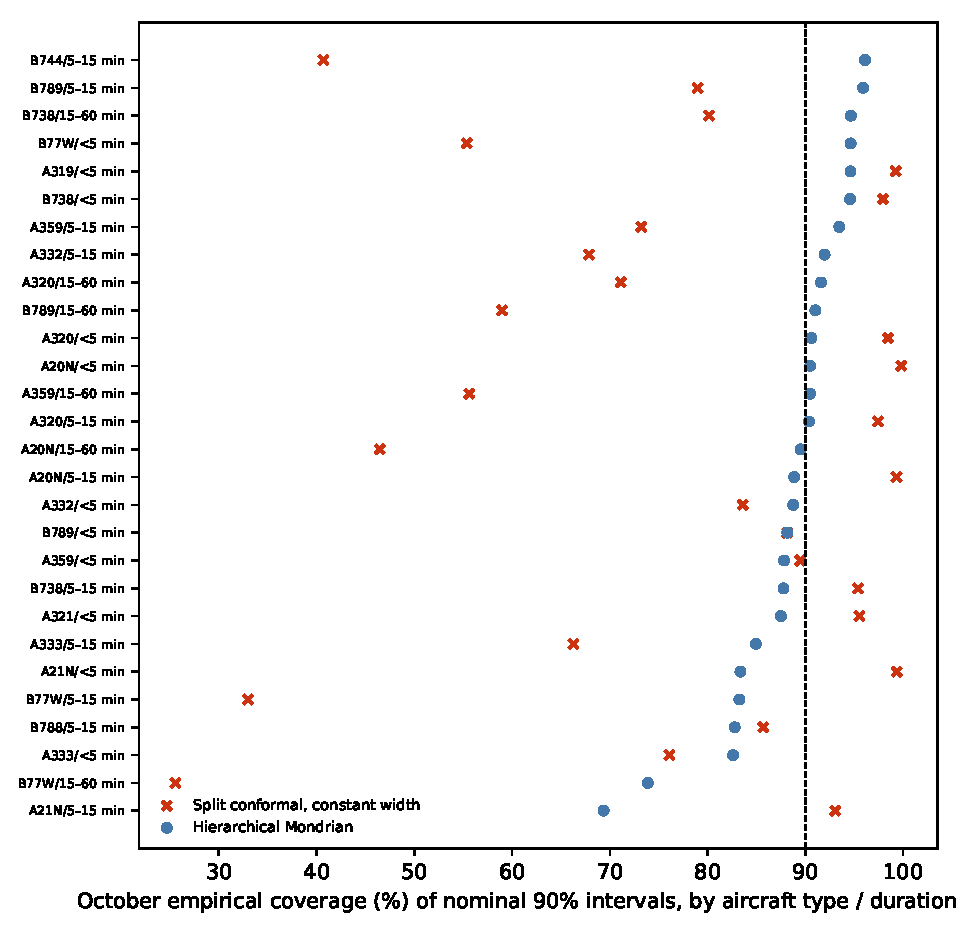
\includegraphics[width=\linewidth]{cell_coverage.pdf}
\caption{Empirical coverage of nominal 90\% intervals in each eligible aircraft-type/duration cell (HGB full point model).}
\label{fig:cells}
\end{figure}

\begin{figure}[t]
\centering
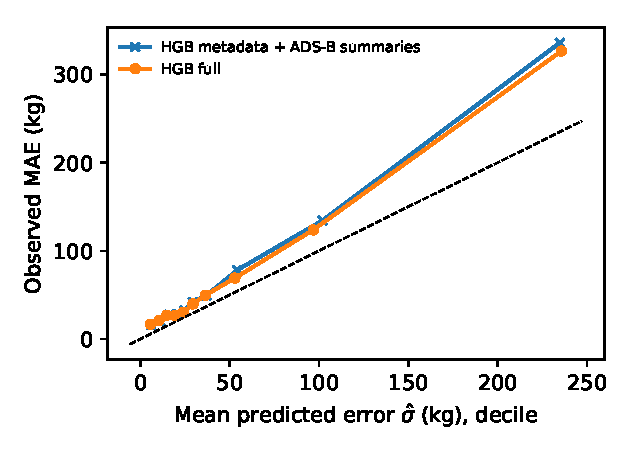
\includegraphics[width=.62\linewidth]{risk_deciles.pdf}
\caption{Observed MAE against mean predicted error $\hat\sigma$ by decile on October 2025.}
\label{fig:deciles}
\end{figure}

\subsection{Representation-aware release}
Table~\ref{tab:selection} and Fig.~\ref{fig:frontier} show the release trade-off at the 75\% target. With risk ranking only, the reference releases \longCovHgbMetadataAdsbRiskOnly{}\% of 15--60-minute intervals and \bSevenCovHgbMetadataAdsbRiskOnly{}\% of B744 intervals while representing \fuelShareHgbMetadataAdsbRiskOnly{}\% of labelled fuel; the 50\% floor raises these to \longCovHgbMetadataAdsbRepresentationFloor{}\%, \bSevenCovHgbMetadataAdsbRepresentationFloor{}\% and \fuelShareHgbMetadataAdsbRepresentationFloor{}\% at an accepted-MAE cost of \floorCostHgbMetadataAdsb{}\,kg. For the physics-residual model the same floor costs \floorCostHgbResidualPhysics{}\,kg (accepted MAE \accMaeHgbResidualPhysicsRiskOnly{} $\rightarrow$ \accMaeHgbResidualPhysicsRepresentationFloor{}\,kg) while representing \fuelShareHgbResidualPhysicsRepresentationFloor{}\% of labelled fuel. A better point model therefore does not remove the access problem---risk-only release still excludes nearly all long intervals and wide-bodies---and lowers the price of fixing it only slightly; the difference in floor cost between estimators is descriptive and was not tested.

\begin{table}[t]
\centering
\caption{Release policies at the 75\% target on October 2025. Fuel share is the fraction of labelled fuel in released intervals; it requires labels and is an evaluation quantity only.}
\label{tab:selection}
\scriptsize
\setlength{\tabcolsep}{3pt}
\resizebox{\linewidth}{!}{\begin{tabular}{llrrrrrr}
\toprule
Point model & Policy & Released & Acc.\ MAE & Rej.\ MAE & Fuel share & 15--60 min & B744 \\
 & & (\%) & (kg) & (kg) & (\%) & released (\%) & released (\%) \\
\midrule
HGB full (+ kinematics + physics) & Risk ranking only & 75.0 & 32.42 & 195.22 & 26.9 & 1.3 & 2.0 \\
HGB full (+ kinematics + physics) & 50\% group floor & 75.0 & 40.88 & 169.83 & 42.0 & 50.1 & 50.0 \\
HGB metadata + ADS-B summaries & Risk ranking only & 75.0 & 33.23 & 206.42 & 26.8 & 0.7 & 0.0 \\
HGB metadata + ADS-B summaries & 50\% group floor & 75.0 & 42.32 & 179.15 & 41.8 & 50.0 & 50.0 \\
Physics-residual HGB & Risk ranking only & 75.0 & 31.98 & 194.80 & 26.3 & 2.4 & 10.2 \\
Physics-residual HGB & 50\% group floor & 75.0 & 39.81 & 171.30 & 40.6 & 50.0 & 50.0 \\
\bottomrule
\end{tabular}
}
\end{table}

\begin{figure}[t]
\centering
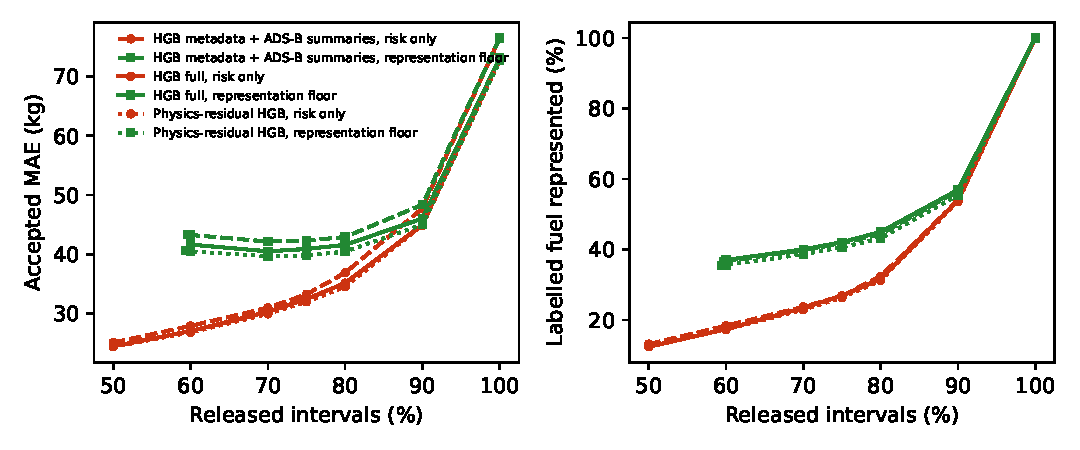
\includegraphics[width=\linewidth]{release_frontier.pdf}
\caption{Release frontier: accepted MAE (left) and labelled fuel represented (right) against release rate for risk-only and 50\%-floor policies.}
\label{fig:frontier}
\end{figure}

\subsection{Flight totals and inventory bias}
Summing interval estimates per flight, the physics-residual model's October inventory bias is \invBiasHgbResidualPhysics{}\% (95\% flight-bootstrap CI \invBiasCiHgbResidualPhysics) against \invBiasHgbMetadataAdsb{}\% (\invBiasCiHgbMetadataAdsb) for the reference and \invBiasOpenapPhysics{}\% for the uncalibrated prior; mean absolute flight-total error is \flightMapeHgbResidualPhysics{}\% versus \flightMapeHgbMetadataAdsb{}\% (type-scaled OpenAP: \flightMapeOpenapCalibrated{}\%). Both learned models' inventory-bias intervals include zero. These totals cover only the labelled intervals of each flight, not whole-flight fuel.

\subsection{Pre-registered hypotheses}
H1 (HGB full improves October MAE with a Holm-adjusted CI excluding zero) is supported. H2 (physics-informed models beat the reference on most withheld types) is supported for HGB full and the physics-residual model but not for the type-scaled prior taken type by type. H3 (Mondrian intervals $\geq$85\% in every eligible cell) is not supported. H4 (a smaller floor cost for HGB full than for the reference) holds descriptively (\floorCostHgbFull{} vs.\ \floorCostHgbMetadataAdsb{}\,kg), with a difference too small to matter in practice.

\section{Discussion}
\paragraph{What the physics prior buys.}
On pooled October data the physics-informed learners improve MAE by \relGainHgbFullOct{}\% (HGB full) and \relGainHgbResidualPhysicsOct{}\% (physics-residual), and the ablation locates that gain in three OpenAP features rather than in the many kinematic summaries. Their clearer value is on withheld aircraft types, where a one-hot type encoding has nothing to offer and pooled held-out MAE falls by \lotoRelGainHgbFull{}\% and \lotoRelGainHgbResidualPhysics{}\%, respectively. This matches the motivation of domain-generalising fuel-flow models~\cite{jarry2025unseen}, obtained here with a public performance model and no proprietary data. The uncalibrated prior is biased because mass and wind are unknown, which is why type scaling and residual learning are both needed, and the gain is not uniform: types with close relatives in training gain little or lose.

\paragraph{Uncertainty must be read per cell.}
A single marginal coverage figure would have rated all three interval methods as adequate. Only cell-level evaluation exposes that constant-width intervals under-cover long wide-body intervals and over-cover short narrow-body ones. Error-scaled and hierarchical Mondrian calibration remove most of this imbalance without new theory, but neither achieves cell-wise validity under a forward temporal shift; small calibration cells for rarer wide-bodies remain the binding constraint, and more calibration data or shift-aware methods~\cite{tibshirani2019weighted,gibbs2023conditional} are needed.

\paragraph{Release policies change the sample.}
Better accuracy lowers but does not eliminate the cost of representation floors. We recommend that any study releasing a filtered subset of open-data fuel estimates report, as here, the released fraction per duration bin and per aircraft type together with accepted and rejected error.

\paragraph{Limitations.}
Labels are ACARS fuel-on-board differences, not measured fuel flow, and \shortOct{}\% of October intervals are shorter than the five-minute lower bound stated by the publisher. Winds, take-off mass, payload and engine variant are absent; ground speed stands in for true airspeed. October was inspected during development of the inherited reference, so no claim of sealed confirmation is made. Routes and operators overlap between periods, and the benchmark covers a single year and a European-centric network. Hyperparameters were fixed rather than tuned, which is conservative for all learned models. The release rule is a deterministic greedy quota, not an optimal policy, and the ``labelled fuel share'' can only be computed where labels exist.

\section{Conclusion}
On the PRC~2025 benchmark, a type-scaled OpenAP prior with learned residual corrections improves forward-test accuracy modestly but significantly over a metadata+ADS-B gradient-boosting model, and transfers substantially better to most withheld aircraft types. Cell-level conformal evaluation shows that marginal coverage hides large under- and over-coverage across aircraft-type$\times$duration cells; error-scaled and Mondrian calibration reduce but do not eliminate it under temporal shift. Risk-only release of 75\% of intervals still drops nearly all long intervals regardless of point-model quality, and a representation floor restores access at a cost of \floorCostHgbResidualPhysics{}--\floorCostHgbMetadataAdsb{}\,kg accepted MAE across estimators. The pipeline, configuration hashes and result files are released so that each reported number can be regenerated.

\subsubsection{Data and code availability.}
The dataset is public under CC~BY~4.0~\cite{zenodo_prc2025}. Code, configuration (\texttt{research\_q1/configs/journal\_study.json}), the result file (\texttt{research\_q1/outputs/journal-study.json}) and this manuscript's generator are in the project repository on branch \texttt{q1-research-extension}.

\subsubsection{Disclosure of interests.}
The authors have no competing interests to declare that are relevant to the content of this article.

\bibliographystyle{splncs04}
\bibliography{references}

\end{document}
